For the estimation of the rigid concepts the \acrfull{tps} mass and the structural mass estimates are combined to yield a single decelerator system mass value. This estimation is based on reference missions rather than structural models as employed for the mass estimates of the inflatable concepts. Steinfeldt \cite{Steinfeldt2009} provides one such mass estimate for a high-mass Mars entry concept. Two concept are considered: a blunt body and a slender body, of which the former is of primary interest for the mission at hand. The reference missions used in Steinfeldt's analysis are all of the blunt body type, similar to the rigid concept considered in this report. As such it is considered applicable to the rigid concept considered in this study. The estimations provided hereafter are all applicable to a blunt body.

Some remarks must be made with regards to the use of these reference missions. Although rigid re-entry missions are plentiful their relevance must be considered. Within this report a re-entry within the Martian atmosphere with a approach velocity of 7 [$km/s$] is considered. Most relevant reference missions are however for a planet different from Mars featuring a different re-entry trajectory. For the re-entry vehicles entering the Martian atmosphere, the approach velocity may still be of a completely different order. Previously executed Martian entries were typically unmanned, featuring a Hohmann transfer to Mars in order to minimize propellent use. The mission at hand features a more direct transfer considering human constraints yielding different approach velocities \cite{Laub2004}. As such the mass estimation should incorporate to some extent the thermal and structural loading of the mission trajectory.

The estimation provided by Steinfeldt takes this into account, dividing the estimation into three different parts: the forebody thermal protection system mass, the forebody structural mass and the back shell structural and thermal protection system mass estimate. The estimation takes into account the size of the concept by using the vehicle total mass at the start of the re-entry \gls{sym:m0}. The heat load is taken into account by using the heat load \gls{sym:Q} and the structural loading is taken into account by using the peak dynamic pressure (\gls{sym:q}).

The mass estimate for the forebody thermal protection system is based on the heat load \gls{sym:Q} and is provided based on empirical analysis by \cite{Laub2004} in Eq.\ref{eq:tps_heat}\cite[p.7]{Steinfeldt2009}:

\begin{equation}
\gls{sym:mheat} = (0.00091Q^{0.51575})\gls{sym:m0}
\label{eq:tps_heat}
\end{equation}

The mass estimate for the forebody structure is similarly given by Eq.\ref{eq:m_structure}\cite[p.7]{Steinfeldt2009} depending on the peak dynamic pressure:

\begin{equation}
\gls{sym:mstructure} = (0.0232 \gls{sym:q} ^{0.1708} ) \gls{sym:m0}
\label{eq:m_structure}
\end{equation}

Applying the empirical relations with a design entry mass of $\gls{sym:m0} = 10000$ [$kg$] yields the relations as shown in Fig.\ref{fig:rigid}.

\begin{figure}[h]
	\centering
	\begin{subfigure}[b]{0.49\textwidth}
	\centering
	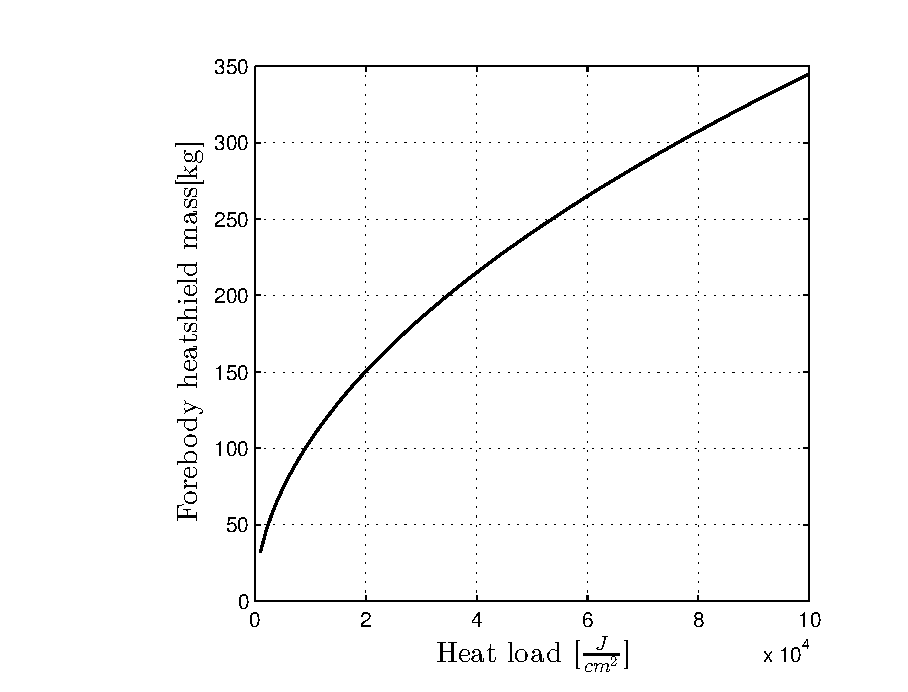
\includegraphics[width=1.0\textwidth]{Figure/rigidheat.eps}
	\caption{Empirical relation for the forebody heat shield mass} 
	\label{rigidheat}
	\end{subfigure}
	\begin{subfigure}[b]{0.49\textwidth}
	\centering
	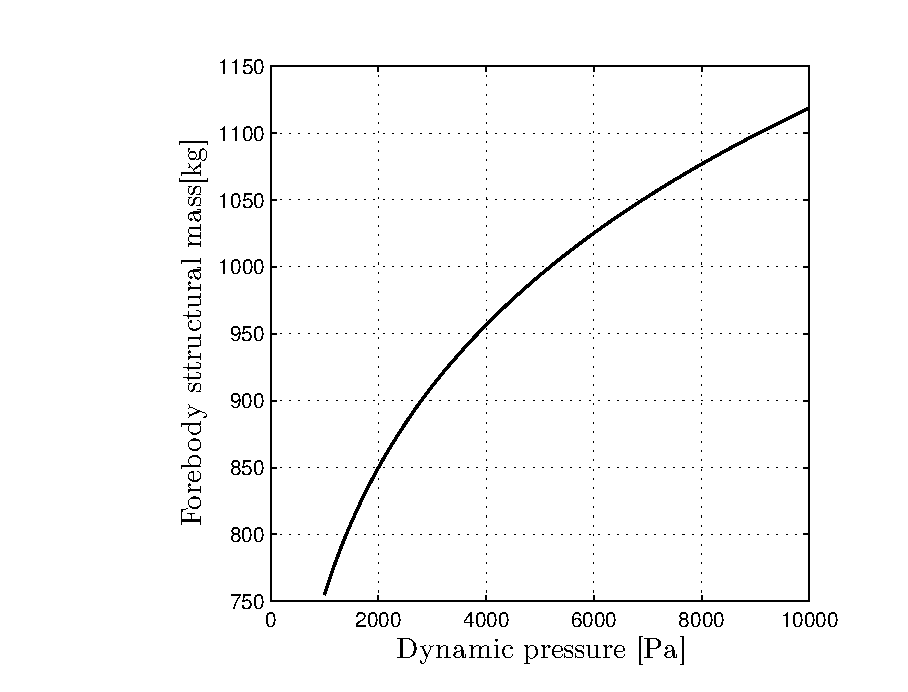
\includegraphics[width=1.0\textwidth]{Figure/rigidstruct.eps}
	\caption{Empirical relation for the forebody structural mass} 
	\label{fig:rigidstruct}
	\end{subfigure}
	\caption{Empirical relations for the forebody mass of a (blunt) rigid concept}
	\label{fig:rigid}
\end{figure}

Fig.\ref{fig:rigid} provides an estimate of the sensitivity of decelerator mass with regard to trajectory, reflected by peak dynamic pressure and heat load. This allows for a first order estimate of the mass of the rigid concept.

Moreover, different from the inflatable concepts a rigid design features an additional backshell structure \cite{Hughes2005}. This backshell is required since the thermal loads are also incurred on the backside of the structure. Steinfeldt suggest a value of 14\% of the total re-entry vehicle mass for the whole backshell thermal protection system and backshell structure \cite{Steinfeldt2009}. This would yield a backshell mass of 1400 [kg] for the rigid concept at hand. The 14\% value should however be considered with care as there is no dependence on the thermal loads and structural loads in any form. Moreover it should be noted that part of this backshell structure may reduce the structural mass of the payload module.

Although the empirical relations stated above should be considered with strict care, a conclusion about the rigid concept can be made. Considering the best case scenario in terms of thermal and structural loads, the rigid concept will not be able to fulfil requirement of a maximum total decelerator mass of 1000 [kg]. Combining the above stated relations for the forebody heat shield mass, forebody structural mass and the backshell mass yields a value (way) above the 1000 [kg] requirement.

Moreover the 1000 [kg] mass requirement is for the whole decelerator concept. This also includes a control system which is not included within this mass estimate further reducing the viability of the rigid concept. 

This result is in line with conclusions reached by Cianciolo et al \cite{Cianciolo2010} and Cassapakis \cite{Cassapakis1995} that inflatable structures provide a weight advantage with respect to a rigid concept.

Therefore the rigid concept is deemed inapplicable in terms of the mass requirement, due to its violation of the 1000 [kg] limit imposed on total decelerator mass. This result is in line with conclusions reached by Cianciolo et al \cite{Cianciolo2010} and Cassapakis \cite{Cassapakis1995} that inflatable structures provide a weight advantage with respect to a rigid concept. As such, no further mass analysis for the rigid concept is performed.

The mass is evaluated at a heat load of 4150 [$\frac{J}{cm^2}$] from Chapter of \ref{ch:thermtool}, which is considered a relatively low value keeping in mind that a single orbit is shared by the rigid and inflatable concepts at this point. This is combined with a peak dynamic pressure of 2400 [Pa] following the selected orbit from Chapter \ref{ch:astrocontrol} yields the mass estimate as in Table \ref{tab:strucmassrigid}

\begin{table}[h]
\centering
\caption{Rigid concept structural \& thermal mass estimate}
\begin{tabular}{|l|l|l|l|l|}
\hline
\textbf{Component {[}-{]}}                                                                                & Forebody heat shield & Forebody structure & Backshell & Total \\ \hline
\textbf{Mass estimate {[}kg{]}}                                                                          & 877           & 668          & 1400             & 2945        \\ \hline
\end{tabular}
\label{tab:strucmassrigid}
\end{table}

 


